\documentclass[amssymb]{revtex4}

\usepackage{graphicx,dcolumn,bm,amsmath,amssymb,color,bm}



\begin{document}



\newcommand{\bs}{ {\bf s} }


\section{Nanoparticle liquid crystals}

Matter composed of anisotropic building blocks (e.g. rod- or disk-shaped mesogens) display structural and dynamic aspects that are much richer than their spherical counterparts. Their key asset is that the interactions -- be they of a direct nature or represented by some potential of mean force -- are intrinsically dependent on the orientations of the constituents. A prominent manifestation is the formation of liquid crystals \cite{gennes-prost}. The most basic liquid crystal state is characterized by long-ranged orientational order in which the main particle axes are oriented along a common director (see \fig{introfig1}b and \fig{introfig2}b). Alternatively, the structure may exhibit additional long-ranged positional order in one or two dimensions. For rod-shaped particles, the most common of such lower symmetry phases is the smectic or lamellar phases (\fig{introfig1}c), characterized by a uni-dimensional periodic stacking of membranes in which rods adopt a bi-dimensional fluid-like structure. For discotic particles,   columnar phases usually arise at thermodynamic conditions favoring a partial freezing of the positional degree of freedom. These structures are composed of a bi-dimensional lattice (usually hexagonal) of  columns of stacked disks. Within these columns the particle centres-of-mass are organized in a disordered manner with no long-ranged positional order. It should be stressed that the structures discussed so far represent all but the most basic liquid crystals and that a vast range of supplementary liquid crystalline states can be expected depending on the symmetry properties of the mesogens under consideration. For example,  particle interactions may
reflect shapes with a reduced particle symmetry such as  biaxial, non-convex, or  polar nanoparticles (which lack head-tail-symmetry), represent particles that are chiral (e.g. helices), or any combination thereof. \fig{introfig1}e illustrates the profound impact of the presence of weak particle chirality; the interactions impart a helical precession of the direction of local alignment (referred to as the director) leading to a cholesteric or chiral nematic phase.   

\begin{figure}
\begin{center}
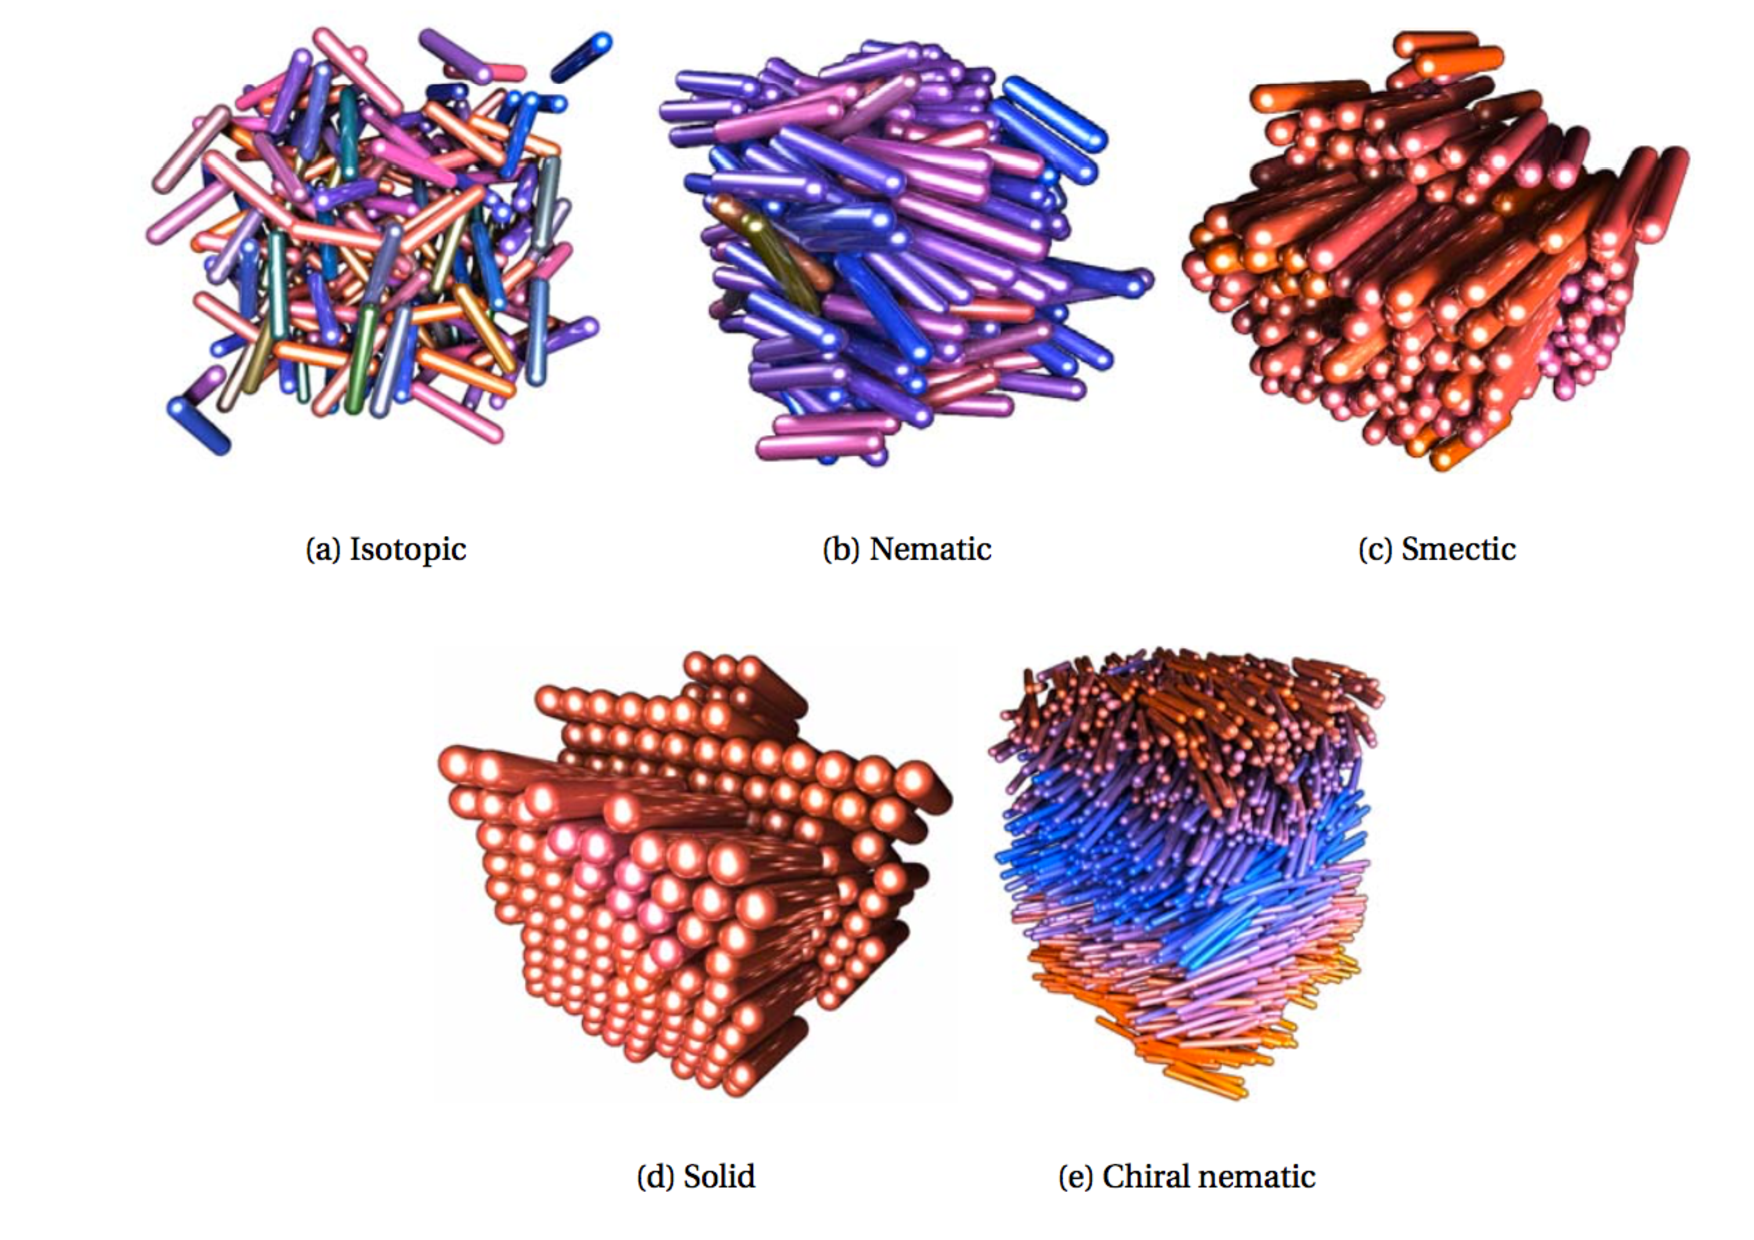
\includegraphics[width= 0.8 \columnwidth]{lcrods}
\caption{ \label{introfig1} Examples of basic liquid crystals formed by rod-like molecules or nanoparticles.}
\end{center}
\end{figure}

 
\begin{figure}
\begin{center}
\includegraphics[width= 0.8 \columnwidth]{lcplates}
\caption{ \label{introfig2} Examples of nematic and columnar liquid crystals composed of plate-shaped particles.}
\end{center}
\end{figure}

The phenomenology of phase transitions enables a broad distinction between molecular liquid crystals, usually referred to as thermotropic liquid crystals and lyotropic ones. For thermotropic systems transformations from one phase to another are primarily of an enthalpic nature since the thermodynamic properties are governed by attractive forces between the molecules (related to van der Waals dispersion, or hydrogen-bonding). Consequently, temperature is the main control parameter and a sequence of states with reduced symmetry (e.g. isotropic, nematic, smectic, solid) is observed upon cooling the system. 

Lyotropic liquid crystals, on the other hand,  consist of nanoparticles or amphiphilic mesogens dispersed in a solvent. Here, the morphology of phases is broadly similar to the one established for thermotropics but the phase behaviour is controlled primarily by the solvent conditions and the concentration of the constituents, rather than temperature. 
Prominent examples are amphiphilic molecules  self-assembling into micellar structures that may adopt complicated topologies ranging from lamellar to bicontinuous cubic phases \cite{seddon1993}. The focus of this thesis  will be on anisotropic colloidal particles whose intrinsic shape, unlike those of micelles, is not subject to fluctuations induced by changes of the solvent composition. Instead the shape is ``quenched''  by the synthetic procedure generating  colloidal suspensions of colloidal particles with a prescribed size and shape.   The relevance of studying nano-particle-based lyotropic liquid crystals  resides in important advances in nano-particle synthesis leading to a plethora of  shapes and interactions with exciting ordering properties \cite{gabriel_davidson2000}. In the natural world, inspiration can be found in self-assembly of filamentous biomolecules  such as DNA \cite{livolantdnaoverview}, and viruses consisting of semi-flexible rod-shaped mesogens \cite{dogic-fraden_fil}. The latter has proven an excellent model system to study fundamental problems in soft condensed matter physics  \cite{dogic2016}. 

An important aspect that sets most lyotropic systems apart from their thermotropic counterparts is that the building blocks are hardly ever identical; they are polydisperse. 
Anisotropic colloids with a distinct  rod- or disk-shape are prone to forming polydisperse mixtures whether the synthesis procedure is controlled or of a natural origin \cite{davidson-overview,davidson1997}. Basic examples range from clay suspension composed of thin sheets with variable diameter \cite{paineau2013},  mineral rods with strong length polydispersity  \cite{buining_jacs1991,vdpol_jcp2008,woolston_jcp2015}, variable-length filamentous biopolymers such as cellulose nanocrystals \cite{lagerwall2014a} or actin \cite{furukawa_actin1993}, to polydisperse carbon-based nanotubes (CNTs) \cite{baughman_cnt2002} and graphene oxide sheets \cite{xu_graphene_LC_2011}.  The implications of size and shape disparity on the equilibrium phase behaviour as well as on the bulk rheological  properties has been the subject of intense experimental and theoretical research over the past decades. 

Most discotic colloidal systems (notably clays) consist of charged disk- or sheet-like mesogens. The disposition of surface charges of clay particles can be very complicated as the chemical composition of the edge surfaces tends to be different from that of the flat surfaces. Further complications arise from the fact that the particle dimensions and surface charge densities are strongly non-uniform. The considerable polydispersity in size, charge and composition inherent to clay systems have severely hampered their fundamental study. 

The focus of the work described in this thesis is to gain a better understanding of some of the fundamental properties underpinning the structure and dynamics of these systems. We shall address three basic themes. The first deals with the profound implications of soft interactions and ``patchiness'', in particular those of a chiral nature, on the mesoscopic order of nematic phases. 
The second theme relates to intricate effects of particle shape, in particular  non-convexity and their effect on the phase behaviour of discotic systems. 
The third theme departs from simple passive systems by moving to so-called {\em active} liquid crystals.  Here,  the building blocks are not passively diffusing across their surroundings but are {\em self-propelled}. This leads to a new class of living  liquid crystals that operate out of thermal equilibrium.    Rather than tackling  the full complexity of the nanoparticles under scrutiny and their intricate surface-chemical properties, we resort to simple models, coarse-grained interactions and tractable theoretical concepts that allow us to acquire important qualitative insights into the (non-)equilibrium self-assembly behaviour of these systems.  As we shall see shortly, the concept of an effective particle  shape often suffices to learn a great deal about the phase behaviour and dynamics of lyotropic systems.  The notion of ``shape matters'' ties in naturally with the concept of entropic phase transitions that we shall discuss next.

\section{Shape matters: entropic phase transitions}

For purely spherical particles,  the discussion about whether a fluid-solid transition can be generated by steep repulsive interactions {\em alone}  or whether atractive forces are a prerequisite dates back to the fifties of the previous century. Using computer simulations  Alder, Wainwright and others \cite{ALDER57,WOOD57} were the first to show that freezing does occur in a fluid of purely hard spheres. Subsequent work by
Hoover and Ree \cite{HooverRee} confirmed that if the hard-sphere packing fraction  
exceeds 49.4 \% a fluid  spontaneously freezes into a crystalline 
solid phase with a packing fraction of 54.5 \%.
Later on, computer simulations by Frenkel {\em et al.}  reported the spontaneous formation of
of smectic and columnar liquid crystals upon densifying systems of respectively hard rods \cite{Frenkel88} and 
 hard platelets \cite{frenkellc,Veerman}.  These types of ordering transitions are usually referred to as entropic phase transition for reasons that become clear if we realize that 
 the equilibrium state of a system kept at constant temperature $T$ is found  from minimizing the Helmholtz free energy $F$:
\begin{equation}
F = U -TS
\label{futs}
\end{equation}
where $S$ denotes the total entropy of the system and  $U = \sum_{i \neqj} u_{ij}$ is the internal energy assuming this quantity to be defined as a pairwise addition of interparticle potentials $u_{ij}$ between particles $i$ and $j$.  If the interactions are strictly hard, then $u_{ij} \rightarrow \infty$ if the hard cores of the objects overlap and $u_{ij} = 0$ otherwise. Invoking Boltzmann statistics, i.e. the probability of finding a particle configuration of energy $U$ is given by $\exp( -U/k_{B}T)$ (where $k_{B}$ denotes Boltzmann's constant), then immediately tells us that {\eny any}  allowable configuration must consists of non-overlapping particles with associated internal energy $U=0$. Clearly, temperature $T$ then becomes completely irrelevant and a minimization of the free energy simply amounts to a maximization of the entropy.  
Of course, the argument that ordered states (e.g. a crystal of hard spheres or an aligned fluid of hard rods) can become thermodynamically stable wth respect to an orderless isotropic fluid based on {\em entropic consideration alone} seems counterintuitive at first since one is tempted to associate ordered states with a lower entropy rather than a higher entropy.  

\begin{figure}
\begin{center}
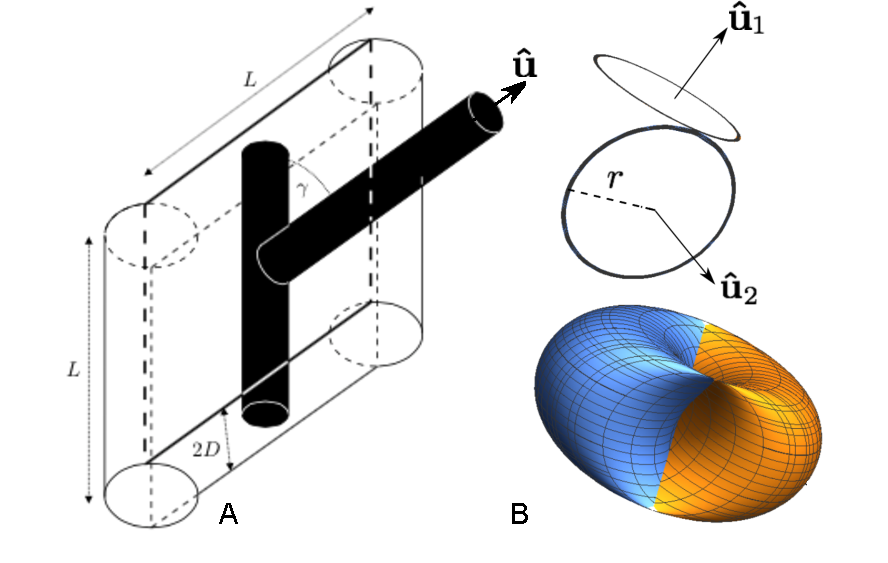
\includegraphics[width= 0.7 \columnwidth]{rodin}
\caption{ \label{introfig3} (A) Illustration of the excluded volume of two cylindrical rods  of length $L$ and diameter $D$ at mutual orientation $\gamma$. Rod alignment leads to a strong reduction of the excluded volume represented by the lozenge-shaped figure. (B) The excluded-volume figure of a pair of inifinitely thin hard rings is much more complicated due to the non-convexity and interpenetrability of the particles.  The consequences for the ordering properties within the context of Onsager's theory will be demonstrated in Chaper 4.}
\end{center}
\end{figure}

That this is not necessarily the case is most clearly illustrated by considering the so-called {\em free volume}  which is the available portion of translational phase space each particle is allowed to explore. Naturally, this free volume is maximal in a dilute isotropic fluid and minimal (virtually zero) if the particles are arranged in a close packed lattice. At intermediate, liquid states,  the free volume will be severely compromised as the particles becomes increasingly crowded.  For hard spheres, there is a critical packing fraction where the particles will be able to better explore translational phase space by adopting an (fcc) lattice arrangement than they would if liquid order were maintained at the same packing fraction. In other words, in crowded conditions,  a solid-like arrangement of spheres will correspond to a higher entropy than a liquid of equal packing packing. This implies that the solid state is thermodynamically favored in these conditions.    

The general mechanism underpinning  entropic phase transitions can therefore be understood as follows:
although the particles lose entropy because the density -- in terms of orientational and/or positional degrees of freedom --
is no longer uniform, this loss is more than offset by a simultaneous gain of translational
entropy, i.e.  the available space per particle -- the average free volume -- increases as the particles align into a nematic fluid or freeze into
a crystal lattice. 
In Chapter 4 we will demonstrate a subtle display of the ordering properties of hard rings (see \fig{introfig3}B) where non-convexity and interpenetrability can lead to surprising phase behaviour.  We reiterate that  the non-trivial self-assembly of these shape-persistent rings \cite{avendano2016} is of purely entropic origin and can be rationalized from geometric considerations alone \cite{wensink_avendano2016}. 


\section{Onsager's theory and beyond}

Onsager's key insight was that the ordering transition for rodlike mesogens, the isotropic-to-nematic transition, is indeed an entropic one and can be analyzed based on entropic arguments alone. Rather than embark on technical exposition of his theory (the reader is referred to Onsager's original paper \cite{onsager} as well as some excellent reviews \cite{vroege92,allenevans} for details) we will attempt to give an intuitive sketch of the main ingredients.  Onsager's theory basically hinges on two principal entropic quantities that are competing with each other.   Let us assume an ensemble of slender rigid needles in a fluid state of uniform particle density $\rho = N/V$ at a fixed volume $V$ and temperature $T$, and focus on the orientational phase space the rods adopt in a fully isotropic and nematic configuration. If we associate each rod orientation on the unit sphere as a separate state we may associate and orientational entropy defines as the ratio of the number of explorable orientational states:  
\begin{equation}
\frac{S_{or}}{N} \sim k_{B} \ln ( \mbox{\# {\small orientational states}})
\label{sor}
\end{equation}
Since in a nematic phase the rod orientation vectors are strongly restricted along either poles of the unit sphere we infer that the orientational entropy $S_{or}$ of a nematic is {\em always} smaller than that of an isotropic fluid at comparable particle concentration. The next consideration concerns the {\em free volume} of an ensemble of rods. Thus, in addition to the orientational entropy there is a configurational entropy, basically quantifying how much translational phase space each rod can explore. This entropy is most conveniently expressed in terms of an {\em excluded volume} and reads:
\begin{equation}
\frac{S_{free}}{N} \sim -k_{B} \frac{V_{excl}}{V}
\label{strans}
\end{equation}
The key approximation that makes Onsager's theory both insightful and tractable is to consider only pair-interactions between slender rods (the so-called second virial approximation) in which case the average free volume can roughly be expressed as a sum of independent pair excluded volumes: 
\begin{equation}
V_{free} \sim \frac{N}{2} \langle v^{ij}_{excl} \rangle_{\mbox{\tiny orientational states of rods i and j}} 
\end{equation}
The meaning of the excluded volume is clarified in \fig{introfig3}. Considering long hard rods we immediately infer that the {\em excluded} volume (indicated by the lozenge-shaped figure) is  strongly orientation-dependent;  it is  greatly reduced when the rods align (such as in the nematic state) compared to  random (isotropic) orientations  where ``end-to-side" pair configurations are more frequent.  The smaller the excluded volume swept out as the cylinders move around with their impenetrable surfaces  in close contact, the greater the free volume and the higher the translational entropy. While nematic order always lowers the orientation entropy it  in fact increases the excluded volume entropy. It is precisely this trade-off between different entropic contributions that underpins the entropic transitions discussed in the previous paragraph. The critical packing fraction at which an isotropic-nematic ordering can be expected roughly corresponds to the situation when the bare particle volume is of the same order as its average excluded volume, i.e.:
\begin{equation}
\phi_{IN} \propto \frac{\mbox{{\small volume per particle}}}{\mbox{{\small average excluded volume per particle}}}
\end{equation}
Simple scaling considerations for thin cylinders then prompt us to infer that the volume scales as $\propto LD^{2}$ whereas the excluded volume typically obeys $L^{2}D $. Whence: 
\begin{equation}
\phi_{IN} \propto \frac{D}{L}
\end{equation}
Clearly, the more slender the rods (large $L/D$) the lower the critical packing fraction at which the transition can be expected. Strictly, in the Onsager limit $L/D \rightarrow \infty$  the transition occurs in the ultra-dilute regime where a pair-interaction-only approximation seems entirely justified.  

Onsager's theory has been tremendously helpful in understanding the equilibrium properties of rodlike mesogens and, to a much lesser extent, discotic particles where the second-virial assumption is a much more severe approximation. 
 It should, however,  be plain that Onsager's arguments are no longer applicable to dense fluids of hard spheres (e.g. to describe the entropic fluid-solid transition) where many-body correlations prevail. These strongly correlated systems call for much more sophisticated considerations from liquid state theory \cite{singh_pr1991,likos_pr2001} or density functional  theory \cite{lowendft} that we will not discuss in this work. 


Attempts to go beyond Onsager's   second-virial approach have met with variable success \cite{harnau_mp2008}. These
approaches usually involve integral equation or geometric density
functional methods whose applicability is often restricted to isotropic
fluids \cite{costa_mp2005,cheung2008}, models with parallel or restricted
orientations \cite{harnaurowan} or particles with vanishing thickness
\cite{esztermann2006,harnaucosta}. A  generalisation of the fundamental
measure approach towards arbitrarily shaped hard convex bodies provides a
potentially promising avenue to address more realistic models for liquid
crystal ordering \cite{hansengoos_mecke2009}.  The influence of higher-body
correlations can in principle be assessed numerically \cite{masters2008}
(at least for isotropic systems) but the convergence of the virial
expansion for the free energy is not guaranteed for dense fluids of hard
cut-spheres \cite{you_jcp2005}. Alternatively, Scaled Particle Theory (SPT)
can be used to incorporate higher virial terms in an indirect manner \cite{savith}.

Going back to the experimental systems of nanorods and platelets mentioned in the beginning it is obvious that a simple hard-particle picture is often too simple to arrive at a satisfactory description of the systems under consideration and that various extensions and modifications of Onsager's theory are necessary.  The most topical ones involve attempts to  account for:
\vspace{0.3cm}
\begin{enumerate}
\setlength\itemsep{1em}
\item Multicomponent mixtures of rod, disks, board-shaped or non-convex particles
\item Non-uniform systems (smectic, columnar phases, interfaces, effect of solid substrates)
\item Effect of external aligning (electromagnetic) fields
\item Semi-flexibility 
\item Electrostatic interactions and other long-ranged ``soft" interactions (e.g. depletion attraction)
\item Chirality
\item Activity, self-propulsion and other non-equilibrium conditions (e.g. shear flow)
\end{enumerate}
\vspace{0.3cm}

\noindent Needless to say that considerable progress has been made along these lines since Onsager's original publication and it would go way too far to review all these developments within the scope of this work. In the main body of this work we will illustrate the rich phenomenology brought about by some of the topics listed above.   The role of chirality (Topic 6) on the mesostructure of nematic phases will be extensively discussed in Chapter 2, while the subtle effect of electrostatic repulsion and intrinsic soft ``patchiness" of rod- and plate-shaped particles (Topic 5) will be discussed in Chapter 3. In Chapter 4 we will demonstrate the surprising effect of shape non-convexity (Topic 1) on the phase behavior of hard anisotropic particles. We hope that these examples will convince the reader of the predictive power and versatility of Onsager's second-virial theory even when applied beyond the strict bounds of applicability as formulated in his original paper.


\section{From hard to soft interactions}


While the seminal view of Onsager that the repulsive inflexible core of a particle gives rise to orientationally ordered phases is now very well established, the specific nature of the dispersive and polar interactions can have an important influence on the macroscopic structures that are observed. 
Interactions between nanoparticles in real systems are never truly hard and taking into account the full molecular complexity of the system under scrutiny (nanoparticle surface, composition of the solvent) necessitates a process called {\em coarse-graining} to arrive at manageable model potentials.   

\subsection{Bridging length scales by coarse graining} 

The current best-practice for modelling nanoparticle suspensions is based first on an analysis of molecular interactions, exploring the choice of materials at the molecular scale, and second, on a transfer of this information to the macro-scale through simplified thermodynamic or statistical mechanical models (such as Onsager's theory in case of anisotropic building blocks).
Transferring knowledge from the molecular scale to the macroscopic is  by no means trivial and usually requires a process known as coarse-graining. This is aimed at integrating out the details of the molecules, such as the explicit conformations of a polymer molecule, the precise localization of charges on a polyelectrolyte or hydrogen bonds on a protein, to give simplified potentials describing the interaction between complex nanoparticles. These effective interactions depend only on a limited set of physically relevant parameters. 
Below we will illustrate several examples in more detail. 

\subsection{The spirit of van der Waals}

The presence of additional soft interactions give rise to enthalpic contribution to the free energy that we will account for in the spirit of a simple van der Waals approximation. This presupposes that these soft interaction act as a perturbation to the entropic hard-core contribution, \eq{strans},  discussed previously in the context of Onsager's theory.  The additional internal energy contribution to \eq{futs} takes the form of a simple mean-field correction term \cite{cotter1977,cotter1979,gelbartbaron,vargachiral2006,francomelgar2008}:
\begin{equation}
U \sim  \frac{1}{2} \frac{N^{2}}{V} \left \langle \int_{\mbox{\tiny no core overlap}} d {\bf r}_{ij}  u_{ij}({\bf r}_{ij})  \right \rangle_{\mbox{\tiny orientational states of rods i and j}} 
\label{uvdw}
\end{equation}
where $u_{ij}$ represents a potential of mean force  between the particles and ${\bf r}_{ij}$ denotes their centre-of-mass distance vector. The complicating factor here is that the soft potential depends on the orientations of the nanoparticles and must be integrated over the space complementary to the excluded volume. i.e.  the domain in which the hard cores of the particles do not overlap (see \fig{introfig3} for the case of spherocylinders).   We stress however that this modification is purely technical and that it is straightforward to draw a parallel between the previous expression and the attraction (or cohesion) contribution to the original van der Waals equation of state for a non-ideal gas:
\begin{equation}
\left ( P + \frac{N^{2}}{V}a \right ) (V - Nb) = Nk_{B}T
\end{equation} 
where $a$ corresponds to the bracketed term in \eq{uvdw} which has units [energy $\times$ volume].  Clearly, in case of attractive forces $|  u_{ij} | <0$,  thence $a<0$ and the cohesive intermolecular forces cause a reduction of the pressure $P$. Similarly, $b$ relates to the excluded volume of a spherical particle -- equal to 8 times its bare volume -- and quantifies (albeit only qualitatively) the reduction of free volume with increasing particle concentration. Let us now briefly discuss the origin of some of the long-ranged forces that might be at play in colloidal systems.  

\subsection{Effective  potentials}

\begin{figure}
\begin{center}
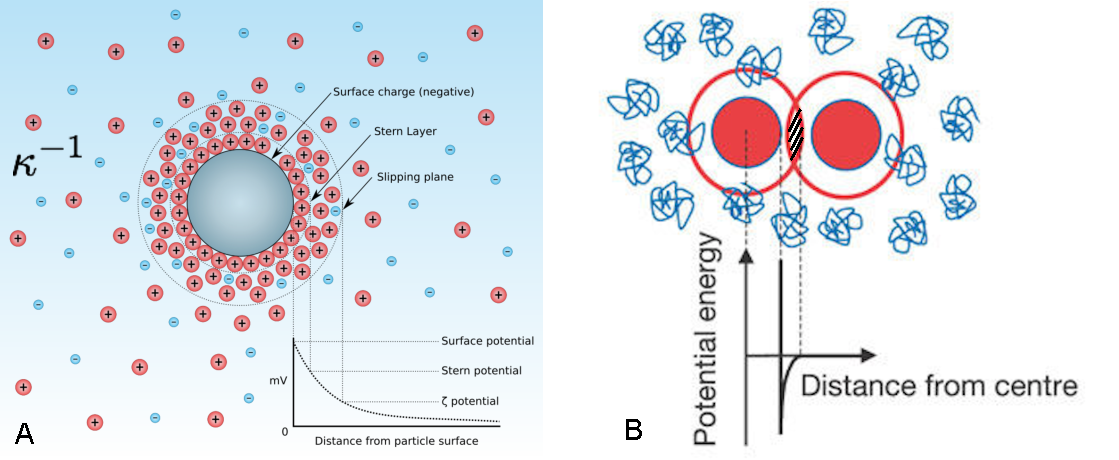
\includegraphics[width= 0.8 \columnwidth]{pomf}
\caption{ \label{introfig4} (a) The presence of surface charges creates an electric double layer around the surface of the nanoparticle surface (a simple sphere in this case). The strongly non-uniform distribution of counter- and co-ions is dictated by the Poisson-Boltzmann equation and gives rise to a soft repulsive potential around the spherical surface. Far from the surface the extent of electrostatic screening is given by the Debye length $\kappa^{-1}$ [\eq{debye}]. (b) The presence of non-adsorbing polymers or other depletions agents (whose size is usually smaller than the spherical nanoparticles) produces an effective attractive potential between the spheres according to the depletion scenario. If the spheres are at close proximity, the polymers are depleted away from the inner space between the spheres in dictated by the overlap of the depletion zones (hatched area). This creates an osmotic imbalance around the spherical surfaces pushing the spheres together.  }
\end{center}
\end{figure}
\subsubsection{{\bf Electrostatics}}
The presence of surface charges creates an inhomogeneous distribution of counter- and co-ions around the surface of the nanoparticle, as illustrated in \fig{introfig4}. This so-called electric double layer imparts a long-ranged repulsive interaction among the particles and can have profound effects on the
ordering properties of colloidal particles \cite{hansenlowen2000}. 
Within the coarse-grained picture one can envisage the effective surface charge, as well as the dielectric properties and ionic strength of the embedding solvent to be the key factors determining the characteristics of this effective interaction.
The precise distribution of the ions around the surface of a charged object is dictated by Poisson-Boltzmann equation in which it is assumed that mutual correlations between the micro-ions can be neglected (i.e. they behave as an ideal gas) and the solvent behaves as a continuum \cite{verwey1955theory}. The highly non-linear equation can be linearized if the surface potential is weak or when attention is restricted to the far-field limit (if the distance between the screened charged surfaces is large). The linearized form is amenable to analytical solution for simple surfaces geometries and the effective potential between two of those surfaces can be calculated in closed form. For example, the effective potential for two simple point-like macro-ions takes the form of a screened Coulomb or Yukawa potential:
\begin{equation}
\frac{u_{ij}}{k_{B}T} = Q^{2} \lambda_{B} \frac{\exp (-\kappa r_{ij})}{r_{ij}}
\label{yukpot}
\end{equation}
 where $Q$ the total or effective surface charge on the particle surface, $\lambda _{B} = e^{2}/4 \pi \varepsilon_{r}k_{B}T$ denotes the Bjerrum length in terms of the elementary charge $e$ and the relative dielectric permittivity $\varepsilon_{r}$ (yielding about $0.7 nm$ for water room temperature). The other important length-scale $\kappa^{-1}$ pertains to the extent of the electric double layer and sets the degree to which the charged surface of the nanoparticle   is screened by the counter-ions:
 \begin{equation}
 \kappa^{2} = 4 \pi \lambda_{B}  \sum_{s=1}^{M} \rho_{s} z_{s}^{2} 
 \label{debye}
\end{equation}

\noindent The screening length is chiefly controlled by the ionic strength via the concentration $\rho_{s}$ of the various ion species $s=1, \dots M$ (each with valence $z_{s}$)  present in the solvent.  
The screened Coulomb potential essentially transforms into the celebrated DLVO potential \cite{verwey1955theory}, widely employed in colloid and interface science, when combined with the  van der Waals potential,  $u_{ij} \sim -u_{0}/r_{ij}^{6}$, describing dispersion attractions that become prevalent when the dielectric contrast between the nanoparticles and the solvent becomes considerable and when the particles are capable of approaching each other closely. This could happen when the electrostatic screening length $\kappa^{-1}$ is much smaller than the typical particle dimension (e.g. in case of added salt) and the van der Waals forces trigger (irreversible) flocculation of the colloids leading to a loss of thermodynamic stability of the colloidal suspension.  
Key challenges arise when attempting to generalize the effective electrostatic potentials to non-isotropic nanoparticles, in particular discotic particles \cite{trizac-weis}. For infinitely slender rods, a simple screened line charge model, as proposed and analyzed by Onsager in his original paper \cite{onsager}, has proven an efficient route to capturing the main effects of electrostatic correlations on the ordering properties of stiff polyelectrolytes \cite{stroobants_mm1986}.   A more detailed discussion about the possibilities and limitations of the screened-Coulomb potential for rod- and disk-shaped particles will be given in Chapter 3. 
In that chapter we provide a simple generalization of Onsager's theory along the lines of \eq{uvdw} that allows us to capture the impact of soft interactions using a superposition of simple spherical segment potentials.
\subsubsection{{\bf Chirality}}
 A similar approach is adopted in Chapter 2 where the distribution of surface charges (or soft sites residing on the rod surface) is distinctly {\em helical} imparting a distinctly {\em chiral} signature onto the effective interactions between the rods.  In this case there is a supplementary soft interaction coupling to the rod orientatation vector ${\bf \hat{u}}$ of each rod $i$ and $j$ (see \fig{introfig3}) and their centre-of-mass distance vector ${\bf r}_{ij}$ through the following generic pseudo-scalar expression:
\begin{equation}
u_{ij} \sim \varepsilon f(r_{ij}) ({\bf \hat{u}}_{i} \cdot {\bf \hat{u}}_{j}) ( {\bf \hat{u}}_{i} \times {\bf \hat{u}}_{j} \cdot {\bf r}_{ij} ) 
\end{equation}
Note that this effective potential is distinctly chiral due to lack of inversion symmetry (the potential changes under a transformation ${\bf r}_{ij} \rightarrow -{\bf r}_{ij} $) while preserving basic head-tail symmetry $u_{ij}({\bf \hat{u}}_{i/j}) = u_{ij}(-{\bf \hat{u}}_{i/j}) $. The microscopic details that are responsible for transmitting chirality can be subsumed into some effective chiral amplitude $\varepsilon$ and decay function  $f(r_{ij})$  expressing the typical range over which chiral forces are transmitted. These properties as well as the impliciation for the helical mesostructure of cholesteric nematic phases (depicted in  \fig{introfig1}e) will be analyzed in detail in Chapter 2.


\begin{figure}
\begin{center}
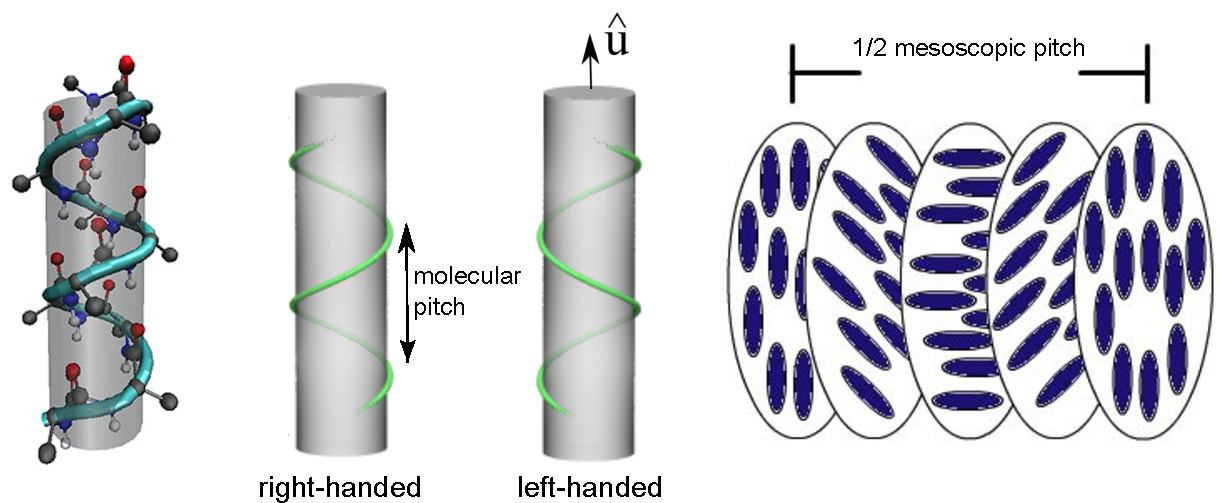
\includegraphics[width= 0.8 \columnwidth]{pitch}
\caption{ \label{introfig8} Interactions between the helical molecular structure of elongated bio-molecules, such as the $\alpha$-helix amino-acid DNA,  could be described on a coarse-grained level using a rod with an effective chiral electrostatic ``patchiness"  in terms of a molecular pitch length and handedness (left or right). The implications of molecular chirality on the helical mesostructure (in particular, the mesoscopic pitch) of chiral nematic phases remains a challenging issue as will be shown in Chapter 2.   }
\end{center}
\end{figure}


\subsubsection{{\bf Depletion}}
Another example of a commonly adopted effective potential concerns the presence of {\em non-adsorbing} agents (note that ions do not qualify as non-adsorbing due to their inherent Coulomb attraction) embedded in an ensemble of much bigger nanoparticles. The effect of the agents on the self-assembly properties of the bigger particles can often be successfully captured by invoking the concept of {\em depletion attraction} \cite{lekkerkerker2011colloids} as illustrated in \fig{introfig4}b. 
Similar to the Yukawa form, while the depletion potential remains relatively tractable for simple spherical particles the quantity  becomes highly non-trivial owing to the intrinsic  orientation-dependence of the depletion zones and their overlap conditions when generalized to suspensions involving rod- or disk-shaped nanoparticles. 
 Within the realm of van der Waals theory (\eq{uvdw}) the depletion attraction between non-isotropic particles could formally be expressed as follows
 \begin{equation}
U \sim  -\frac{1}{2} \frac{N^{2}}{V} \Pi_{dep} \left \langle \int_{
\substack{
\mbox{\tiny no core overlap,} \\ 
\mbox{\tiny depletion zone overlap}
}
} d {\bf r}_{ij}   v^{dep}_{ij}({\bf r}_{ij})  \right \rangle_{\mbox{\tiny orientational states of rods i and j}} 
\label{degen}
\end{equation}
In arriving at this expression,  a simple free-volume concept has been invoked in which the depletion agents are considered to be mutually non-interacting and the effective attraction potential between the nanoparticles is proportional to the overlap volume $v^{dep}_{ij}$ of the depletion zones of particles $i$ and $j$ (see \fig{introfig4}b) and the osmotic pressure $\Pi_{dep}$ exerted by the depletion agents \cite{lekkerkerker2011colloids}.   

\subsection{Entropic patchiness}

Mixing non-isotropic colloidal shapes with non-adsorbing polymers lead to so-called {\em entropic patchiness}; the strength of the attractive depletion force depends on the mutual particle orientation since the overlap volume of the depletion zones is not invariant  with a change of the nanoparticle orientation \cite{petu2017}.
Within the context of this thesis, we wish to underscore that whenever the soft interactions are purely  repulsive, such as in the case of electrostatic-mediated chirality described in Chapter 2  or charged disks considered in Chapter 3, the intrinsic  orientation-dependency of the interactions leads to a {\em patchiness} that is of purely entropic origin. A clear manifestation of entropic patchiness regulated by shape along are the rigid macrocyles discussed in Chapter 4 where  the interpenetrability of the rings may, under certain circumstances, favor face-to-rim configurations over face-to-face ones (see also \fig{introfig3}).


\section{From passive to living liquid crystals}


In the second part of this thesis, we depart from the concept of ordering properties of common nanoparticles and explore the possibilities of using the simple coarse-grained models and effective potentials introduced before to describe so-called active or living  soft matter \cite{2010ramaswamy, marchetti_rmp2013}. 
Analogous to  liquid crystals, the building blocks of living matter are often non-isotropic and many of the basic geometric considerations  carry over to describing basic interaction between motile organisms \cite{baskaran}. For instance, bacteria and other motile microorganisms often possess a rod-like shaped cell bodies with a strong tendency to align when they swim in close proximity to each other(\fig{introfig7}).  Such systems, interacting either directly or indirectly via the medium, are generically capable of emergent behaviour at large scales \cite{2009CoWe,2011KochSub,2009SoAr,2011drescheretal}, leading to swarming or flocking behaviour~\cite{2010kearns,2010ramaswamy} or complex vortical states ~\cite{2000Be,2004DoEtAl,2007SoEtAl,2005Riedel_Science,2008SaintillanShelley}. 


\subsection{Active matter}

The essential difference with common lyotropic liquid crystals is that while the constituents of passive systems are subject to passive Brownian motion due to molecular collisions embedded solvent molecular, active particles are {\em self-propelled}  due to some internal propulsion mechanism.
Examples of active particles are bacteria that are capable of taking up energy from its surroundings and engage in propelled motion through actuation of their flagellae. This type of motion is not persistent but subject to fluctuations, for instance, the flagellae may disentangle and reorient the cell-body through a sequence of run-and-tumble events as illustrated in \fig{introfig6}.   At large time scales the bacterial trajectory can be viewed as the results of an active diffusion process enabling us to make predictions based using well-established stochastic  models \cite{2012pawel_review}. Since each particle carries an ``internal motor" constantly converting chemical energy into mechanical work (propulsion) they operate essentially {\em out of thermal equilibrium}. It should be understood that active systems are different from other classes of driven systems as the energy input is {\em internal} to the medium (i.e. located on each unit) and  does not act at the boundaries or via external fields.


\begin{figure}
\begin{center}
\includegraphics[width= 0.8 \columnwidth]{./FINTRO/randt}
\caption{ \label{introfig6} Many motile bacteria exhibit run-and-tumble behaviour consisting of a run stage in which bundled flagella provide propulsion and a short phase in which the flagellae disentangle and reorient the bacterial cell body (tumbling event). The typical trajectory of a bacterium can be described as an active diffusion process (right cartoon).}
\end{center}
\end{figure}


In view of the strict non-equilibrium nature of these systems,  the tools of classical equilibrium thermodynamics (such as minimization of the Helmholtz free energy \eq{futs}) are no longer appropriate to study their ordering behaviour. Instead,  one must resort to resolving the equations of motion of the individual particles by accounting for the (pair) interactions using simple coarse-grained models. This will be briefly illustrated in the last paragraphs of this chapter.
  
  
  \subsection{System dimensionality}   
 
 Attempts to study active matter using theoretical modelling are often greatly simplified by considering bi-dimensional systems.  The advantage is usually based purely on the ease with which these systems can be visualized. In addition, simulations and other numerical approaches are often less computationally cumbersome in reduced dimensions.  However, inspiration can also be found in many experimental situations where a two-dimensional model description seems  more appropriate.
 For example, self-propelled agents resembling two-dimensional behaviour can be realised in a number of ways including autonomously
navigating bacteria and other microbes confined to free-standing thin films \cite{2007SoEtAl}, moving near a solid surface \cite{mino_clement}  or a liquid-gas interface \cite{2004DoEtAl, 2011Japan},  polar granular rods vibrating on a flat surface \cite{kudrolli,2007NaRaMe}, and even pedestrians moving in complex
environments \cite{Helbing}. Last not least, colloidal dispersions constitute ideal model systems
not only for investigating passive matter \cite{lowen2001,lowen2008} but also 
for living  matter consisting of self-motile units. Over the last decade, a number of distinctly different realizations of active colloidal particles have
been proposed. These include Janus particles  driven by catalytic processes
\cite{baraban,bocquet} or thermophoretic \cite{bechinger}  gradients,  particles propelled by artificial
flagellae \cite{dreyfusbibette} and surface waves \cite{snezhko_prl, snezhko_nature} driven in an external magnetic field. 
Most of these particle are anisotropic, i.e. rod-shaped rather than spherical and their shape is found to play a crucial role in determining the spatio-temporal behaviour  \cite{2006Peruani, Peruani2012}.  Confining systems to quasi-planar geometries allows for a direct visualisation of the particles by means of real-space microscopy and provides  fascinating opportunities to study the single-particle and collective behaviour of micro-swimmers.

 
    
  \subsection{Dry versus wet flocks}
  

  
The role of the medium play an important role and allows a distinction between dry and wet systems.   Indeed, dry flocks can be viewed as a manifestation of a living liquid crystal showing a complex spatio-temporal behavior \cite{1995tonertu_prl} even though the non-isotropic constituents  (birds, insects) are no longer of microscopic size. The same holds for certain wet flocks, such as schools of fish, where the swimming locomotion and the corresponding hydrodynamic interactions between the agents mediated via the embedding solvent (water) plays an important role. In the micro-world, the hydrodynamics of swimming locomotion remains a serious complication in describing interacting micro-organisms. An important distinction between swimming at micro- or macroscopic length scales is that the Reynolds number, defined as 
\begin{equation}
\text {Re} =  \frac{\mbox{{\small inertial forces}}}{\mbox{{\small viscous forces}}} = \frac{L_{0} v_{s}}{\eta}
\end{equation}
is very small in the former case. Taking typical values for the bacterial swimming speed $v_{s} \sim 10 \mu m /s$,  size $L_{0} \sim 1 \mu m $ and kinematic viscosity of water $\eta = 10^{-6} m^{2}/s$ yields $\text{Re} \sim 10^{-5}$.  Locomotion at these ultra-low Reynolds numbers has important consequences for the propulsion and swimming mechanics of bacteria operating essentially in the Stokes'  regime of the Navier-Stokes equation.  As formulated in a beautiful paper by Purcell \cite{1977pu}, the complete dominance of viscous over inertial forces renders the fluid flow instantaneous so that only micro-organisms performing swimming stroke cycles that are {\em time-irreversible} are capable of net propulsion in these conditions (this is coined the ``scallop theorem").

When studying many-particle systems, resolving and intercorrelating the stroke-induced flow field around each particle becomes  a completely impracticable enterprise and one needs to resort to simple, coarse-grained,  pairwise additive potentials that can be employed in computer simulation \cite{putz2010}.
For dense collections of bacteria, there is strong experimental evidence that {\em far-field} hydrodynamical interactions between bacterial cell bodies are far less important than direct collisions, particularly when the bacteria are confined in quasi-2D set-ups where hydrodynamic interactions are strongly screened \cite{2011drescheretal}. Near-field hydrodynamic flows are notoriously difficult to quantify \cite{laugapowers}.  For {\em dense} collections of swimmers, however, it is not unreasonable to assume that  the near-field effects can be subsumed into an effective short-ranged repulsive potential.   This simplification leads to a so-called self-propelled rod (SPR), explained in \fig{introfig9}. The physics generated by this model in relation to real bacterial fluids will be discussed in  further detail in Chapter 5.

  \begin{figure}
\begin{center}
\includegraphics[width= 0.8 \columnwidth]{./FINTRO/acmat}
\caption{ \label{introfig7} Pair interactions between active, self-propelled organisms suggest strong aligning properties. At the many-body scale self-propulsion leads to the formation of non-equilibrium emergent states such as flocks in which the medium plays and important role. Left:  wet flock of sliding myxobacteria.   Right: dry flock of birds.  }
\end{center}
\end{figure}
   



  
  \subsection{Active diffusion in wet flocks: some basic  considerations}

We shall now attempt to briefly sketch how one could go about studying the ordering properties of an ensemble of active particles using considerations from {\em equilibrium} thermodynamics as considered in paragraph 1 of this chapter. Let us denote $P(\bs,t)$ as the probability to find a active particle at a certain position  and orientation, collectively denoted by the generalized coordinate $\bs =\{ {\bf r}, {\bf \hat{u}} \}$ and time $t$. The time-evolution of this probability is described by the following diffusion equation \cite{dhont,2008pawel}: 
\begin{equation}
  \label{eq:ddft}
  \nonumber
  \partial_{t}  P( \bs,t) =
 - {\bf \nabla} \cdot {\bm \overline{\zeta}}^{-1}_{T} \cdot \left ( {\bf j} _{\text{trans}} + {\bf j}_{\text{active}}  \right )  -\zeta_{R} {\bf \hat{\mathcal{R}}} \cdot   {\bf j}_{\text{rot}}  
 \end{equation}
 in terms of a  translational Stokes'  friction tensor ${\bm \overline{\zeta}}_{T}$ and a rotational friction factor $\zeta_{R} $. If we neglect many-body hydrodynamics interactions between the particles, then these quantities encode the single-particle hydrodynamic friction of the particles  governed primarily by their aspect ratio $L/D$ (introduced in Section 1.3). We have implicitly assumed that the system is `wet' and that particles move in the overdamped limit, that is,  we focus at time scales much larger than those associated with solvent relaxation and particle inertia,  so that the propulsion velocity is proportional to some {\em effective} thrust force $f_{t}$ divided by the parallel translational friction each rod experiences as it moves through the fluid: 
\begin{equation}
v_{s} \sim \frac{f_{t}}{\zeta_{\parallel}}
\end{equation}
This defines an active current coupled to the main orientation ${\bf \hat{u}}$ of the self-propelled rods:
 \begin{equation}
{\bf j}_{\text{active}} =  P(\bs , t) f_{t}{\bf \hat{u}}
 \end{equation}
The other two currents encode the correlation between the particles. Within the framework of dynamic density functional theory \cite{marconi1999,archer2004} it is possible to connect these non-equilibrium currents to the {\em equilibrium} excess Helmholtz free energy \eq{futs} in the following way: 
\begin{equation}
{\bf j}_{\text{trans}} =  P(\bs,t) {\bf \nabla }  \frac{\delta  F_{ex}[P]}
      {\delta P (\bs ,t)}  
 \end{equation}
and a similar contribution for the orientational correlations (representing collisional torques): 
 \begin{equation}
{\bf j}_{\text{rot}} = P(\bs,t) {\bf \hat{\mathcal{R}}}    \frac{ \delta F_{ex} [ P] } {\delta P(\bs,t)} 
 \end{equation}
in terms of a rotation gradient operator $\hat{\mathcal{R}}}$. Expressions for the (excess) Helmholtz free energy, which is now an explicit functional of the probability distribution $P$, can be constructed using geometric considerations along the lines of the excluded-volume concept illustrated in \fig{introfig3} \cite{baskaran}.  Typically, this would give an excess free energy of the following form:
\begin{equation}
F_{ex} \sim \frac{1}{2}k_{B}T \int d \bs P(\bs,t) \int d \bs^{\prime} P(\bs^{\prime},t) \Theta (\bs , \bs^{\prime})
\end{equation}
wher the step function $\Theta $ yields unity in case of core overlap and zero otherwise. It is easily verified that the free-volume entropy \eq{strans} is recovered from the above expression for a spatially {\em homogeneous} system where the probability function reduces to $P = (N/V)$ times the orientational probability. 
Needless to say that these quasi-equilibrium approaches to modeling active matter are highly approximative as they do not account for correlations that are generated by the non-equilibrium currents themselves (so called dynamical correlations) or correlations arising from the coupling of the complicated hydrodynamic flow fields generated by the swimmers \cite{laugapowers} (cf. \fig{introfig9}).

  
   \begin{figure}
\begin{center}
\includegraphics[width= 0.8 \columnwidth]{./FINTRO/acrod}
\caption{ \label{introfig9}  (A) A typical bacterial swimmer is {\em force-free} and can be modelled as a simple force dipole consisting of a pushing force and an opposing drag force (red arrows), as demonstrated for the case of a {\em pusher}-type swimmer such as {\em E. Coli} or {\em B. Subtilis}.
The stroke-averaged far-field fluid flow generated around the cell body represents a dipolar field where the average fluid velocity decays with distance as $1/r^{2}$ away from the bacterial body. The black arrow indicates the direction of propulsion.  (B) Dense bacterial fluids of {\em B. Subtilis} confined in quasi-2D chambers are characterized by short-ranged steric repulsions  prevailing  over long-ranged hydrodynamic interactions. (C) Self-propelled rod (SPR) representation of a bacteria of typical aspect-ratio $\ell/\lambda$ consisting of a rigid array of steeply repulsive segments (interacting through a Yukawa potential  \eq{yukpot}) at site-site distance ${\bf r}_{ij}$ and centre-of-mass distance vector ${\bf \Delta r}$. Each rod  is auto-propelled through an overdamped frictional medium via some {\em effective} thrust force $f_{t}$ directed along the main axis ${\bf \hat{u}}$.  }
\end{center}
\end{figure} 
 

\subsection{Shape matters in the biological world}

Building on the considerations above we can propose an equivalent route to studying the ordering properties of active matter by focussing on the trajectories of {\em individual} SPRs.  In the overdamped limit, the positional trajectory of a rod $i$ at coordinates $\{ {\bf r}_{i}, {\bf \hat{u}}_{i}\}$ is dictated by the Langevin equation which essentially represents a balance of the principal forces acting on each rod: 
\begin{equation}
\underbrace{ {\bm \overline{\zeta}}_{T} \cdot \partial_{t} {\bf r}_{i}(t)}_{\mbox{\tiny frictional force}} =  \underbrace{f_{t} {\bf \hat{u}}_{i}(t)}_{\mbox{\tiny active force}}  \underbrace{-\nabla_{i} U (\{ {\bf s}(t) \} )}_{\mbox{\tiny interaction force}}  + \underbrace{{\bf f}_{R,i}(t)}_{\mbox{\tiny stochastic force}}
\label{lar}
\end{equation}
with the latter embodying some random force describing the  Brownian force fluctuations exerted by the embedding solvent molecules.  The active force is explicitly coupled to the rod orientation ${\bf \hat{u}}_{i}$. The interaction force depends {\em implicitly} on the rod orientations and is derived from the total potential energy  $U(\{ {\bf s}(t) \}) = U({\bf r}_{i}(t), {\bf \hat{u}}_{i}(t), \dots, {\bf r}_{N}(t), {\bf \hat{u}}_{N}(t))$ which now depends on the coordinates of {\em all} $N$ rods in the system. We remark that a numerical solution of \eq{lar} in principle enables an exact treatment of the rod-rod correlations beyond the simple second-virial approximation considered thus far. The above equation needs to be supplemented with a similar one describing a torque balance on each rod $i$:
\begin{equation}
\underbrace{ {\bm \zeta}_{R}  \partial_{t} {\bf \hat{u}}_{i}}_{\mbox{\tiny frictional torque }} =   \underbrace{-\nabla_{{\bf \hat{u}}} U (\{ {\bf s} \})}_{\mbox{\tiny interaction torque}}  + \underbrace{{\bf \tau}_{R,i}}_{\mbox{\tiny stochastic torque}}
\end{equation}
In Chapter 5 we will demonstrate that this simulation scheme allows us to study the subtle role  of particle shape on the emergent states of active rods \cite{2012wensinklowen}. Most notably, it turns out that propulsion and short-repulsive interactions (the SPR model) can lead to {\em turbulent} states at high particle concentration and large particle aspect ratio \cite{2012wensink_pnas}. This type of active turbulence is routinely observed in microbial suspensions of {\em Bacillus Subtilis} \cite{2007cisneros}. A detailed analysis of the flow properties of this novel type of {\em low Reynolds number} turbulent flow will be made in Chapter 5. Despite the overwhelming complexity of bacterial locomotion and interactions  we will demonstrate that the main features of the flow field can be described using a simple hard-rod (SPR) model coupled to simple linear, overdamped propulsion. In  Chapter 6 we follow up on our study of particle shape in living liquid crystals by focussing on  varying the particle symmetry of the SPRs. The objective is to investigate the role of broken particle symmetry (polar and non-convex particle shapes) on the emergent behaviour.  We will demonstrate that a broken for-aft symmetry (producing polar swimmers) can dramatically change the mesostructure, depending on whether the particles are propelled along or anti-parallel to the polar symmetry axis. The  respective emergent states correspond to flocking behaviour and colony formation driven by motility-induced phase separation \cite{catestailleur2015}.  These phenomena are a unique consequence of the non-equilibrium, propulsive behaviour of the constituents and are unseen in passive liquid crystals.

\bibliographystyle{unsrt}
\bibliography{lul1}

\end{document}















